\newpage\section{Instrukcja użytkowania aplikacji}
Aplikacja przeznaczona na urządzenia mobilne z system Android w wersji minimum 4.0.3.

\begin{enumerate}
	\item Po uruchomieniu aplikacji wyśietli się menu głowne(rys.1.).
	\begin{figure}[ht!]
		\centering
		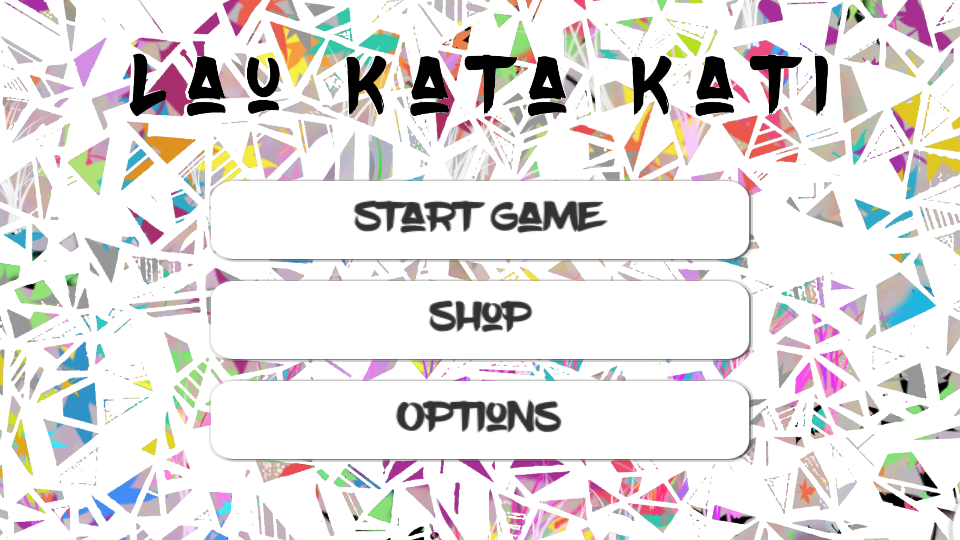
\includegraphics[width=55mm]{img/ekran_glowny.png}
		\caption{Ekran głowny}
	\end{figure}

	\item W menu \textit{„Shop”} istnieje opcja kupna/zmiany skórki pionków za zebrane punkty oraz możliwość obejrzenia reklamy co 20 minut – reklama dodaje 10 punktów (rys.2.).
	\begin{figure}[ht!]
		\centering
		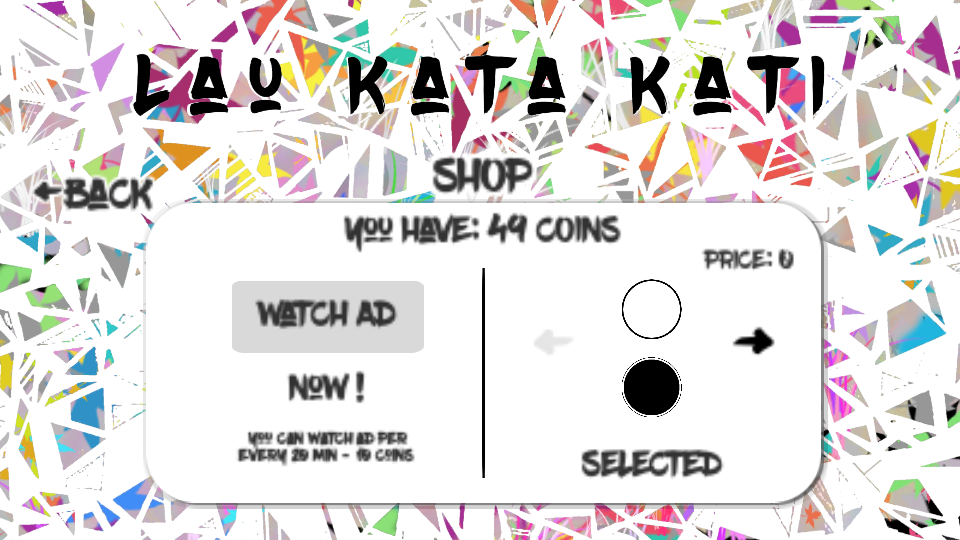
\includegraphics[width=55mm]{img/sklep.png}
		\caption{Ekran sklepu}
	\end{figure}
	
	\item W menu \textit{„Options"} można ustawić poziom trudności maszyny grającej od 1 do 9 (rys.3.).
	\begin{figure}[ht!]
		\centering
		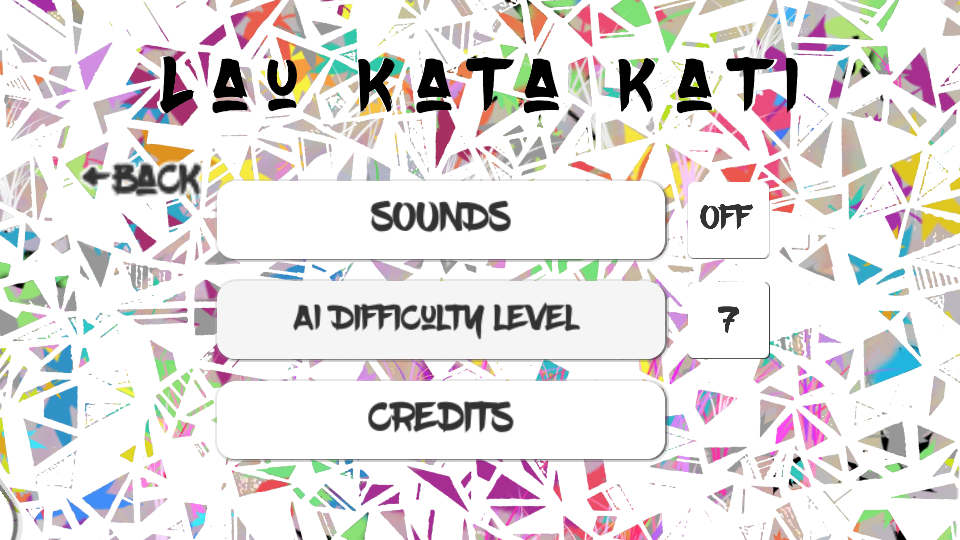
\includegraphics[width=55mm]{img/opcje.png}
		\caption{Ekran opcji}
	\end{figure}
	
	\item Po naciśnięciu \textit{„Start game”} ukażą się trzy tryby rozgrywki (rys.4.):
	\begin{itemize}
		\item \textit{Singleplayer} – rozgrywka przeciwko maszynie grającej,
		\item \textit{Multiplayer} – lokalna rozgrywka dwuosobowa,
		\item \textit{Online Multiplayer} – rozgrywka dwuosobowa przez Bluetooth.
	\end{itemize}
	\begin{figure}[ht!]
		\centering
		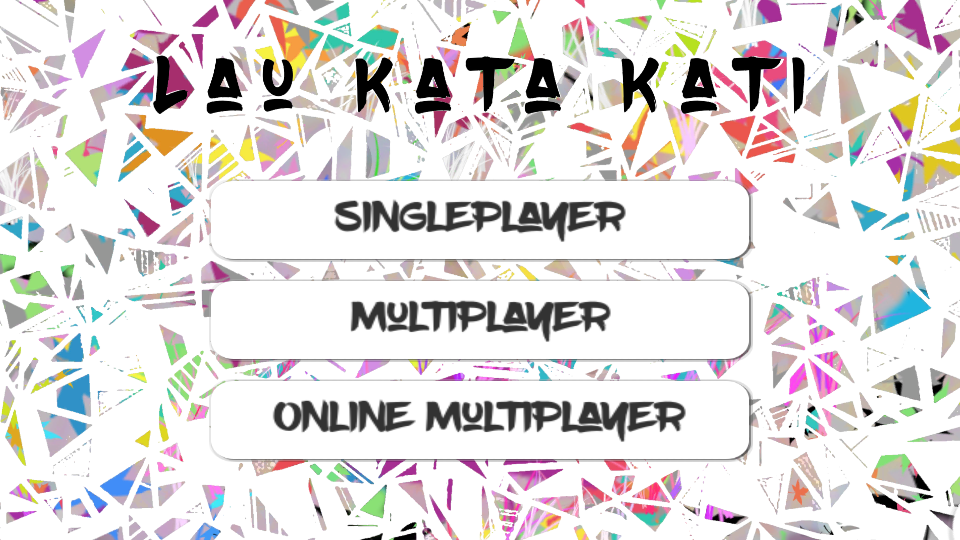
\includegraphics[width=55mm]{img/ekran_trybow.png}
		\caption{Ekran wyboru trybu gry}
	\end{figure}

	\item Po wybraniu trybu \textit{„Singleplayer”} zostanie rozpoczęta rozgrywka przeciwko SI (rys.5.).
	\begin{figure}[ht!]
		\centering
		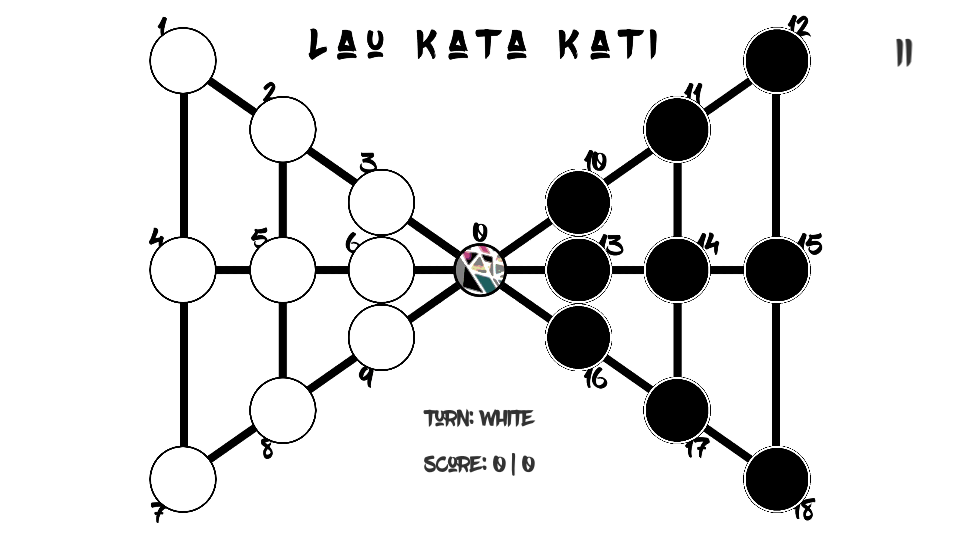
\includegraphics[width=55mm]{img/singleplayer.png}
		\caption{Widok trybu singleplayer}
	\end{figure}

	\item Wybranie trybu \textit{„Multiplayer"} rozpocznie lokalna rozgrywkę multiplayer.
	
	\newpage
	\item Po wybraniu trybu \textit{„Online Multiplayer"} jeden z graczy musi utworzyć serwer gry wybierając opcję \textit{„Server"}. Po utworzeniu serwera gracz drugi łączy się przez Bluetooth wybierając opcję \textit{„Client"}. Rogrywka rozpocznie się po wylosowaniu i przesłaniu tury do klienta (rys.6.). 
	\begin{figure}[ht!]
		\centering
		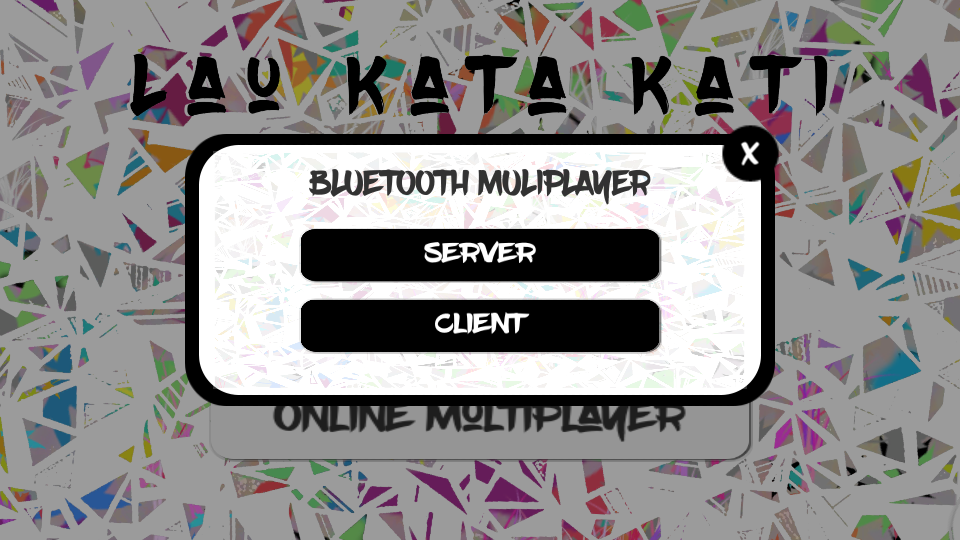
\includegraphics[width=55mm]{img/bluetooth.png}
		\caption{Opcje trybu Online multiplayer}
	\end{figure}
\end{enumerate}